\chapter{高度制御}

高度センサーで高度を計測して,制御する.センサーの性能を測定した.いかにその結果を示す.

今回使用した超音波センサーを図4.1に示す.
\begin{figure}[htbp]
  \begin{center}
   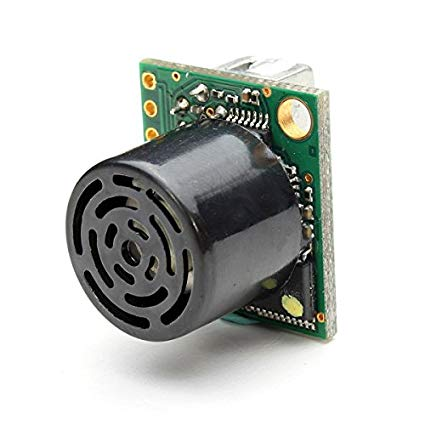
\includegraphics[width=100mm]{img/超音波センサー.jpg}
    \end{center}
  \caption{超音波センサー}
 \label{fig:ensyu3tex}
\end{figure}


\section{超音波センサーの性能確認}

以下に実験手順を示す.

\begin{enumerate}
  \item 距離と出力の確認.
アクリル板を少しずつずらして,距離と出力の関係を確認した.

\begin{figure}[htbp]
  \begin{center}
   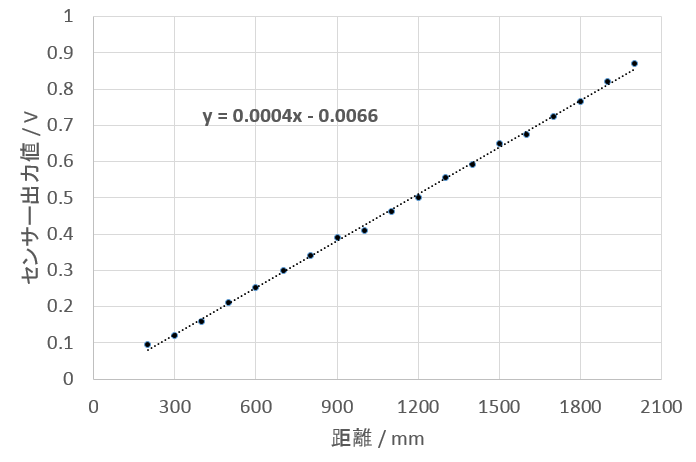
\includegraphics[width=150mm]{img/距離と出力.jpg}
    \end{center}
  \caption{超音波センサーの距離と出力の関係}
 \label{fig:ensyu3tex}
\end{figure}

図4.2より,距離に応じてセンサーの出力値が比例していることがわかる.

  \item 検知範囲の確認.

センサーの検知範囲を確認した.

\begin{figure}[htbp]
  \begin{center}
   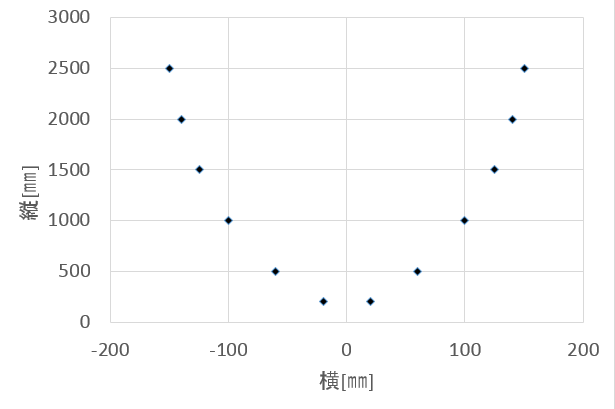
\includegraphics[width=150mm]{img/検知範囲.png}
    \end{center}
  \caption{超音波センサーの検知範囲}
 \label{fig:ensyu3tex}
\end{figure}

図4.3より超音波センサーの音波は広範囲に広がって検知している.
超音波センサーの性能を確認することができた.
\end{enumerate}




\chapter{高度制御のシミュレーション実験}
制御性能をシュミレーションで確認する.

Pythonによって製作された制御シミュレーションCADを用いて,PID制御の比例ゲイン$K_P$,積分ゲイン$K_I$,微分ゲイン$K_D$に値を入れてシミュレーションを模擬実験する.

\section{PID制御}
偏差(目標値と現在値の差)に比例して制御量が増える比例制御(P),偏差がある状態が長時間続くにつれ制御量が増えていく積分制御(I),偏差が急激な変化をするほど制御量が増える微分制御(D)を組み合わせた基本的な制御手法である.
ブロック線図を図5.1に示す.

\begin{figure}[htbp]
  \begin{center}
   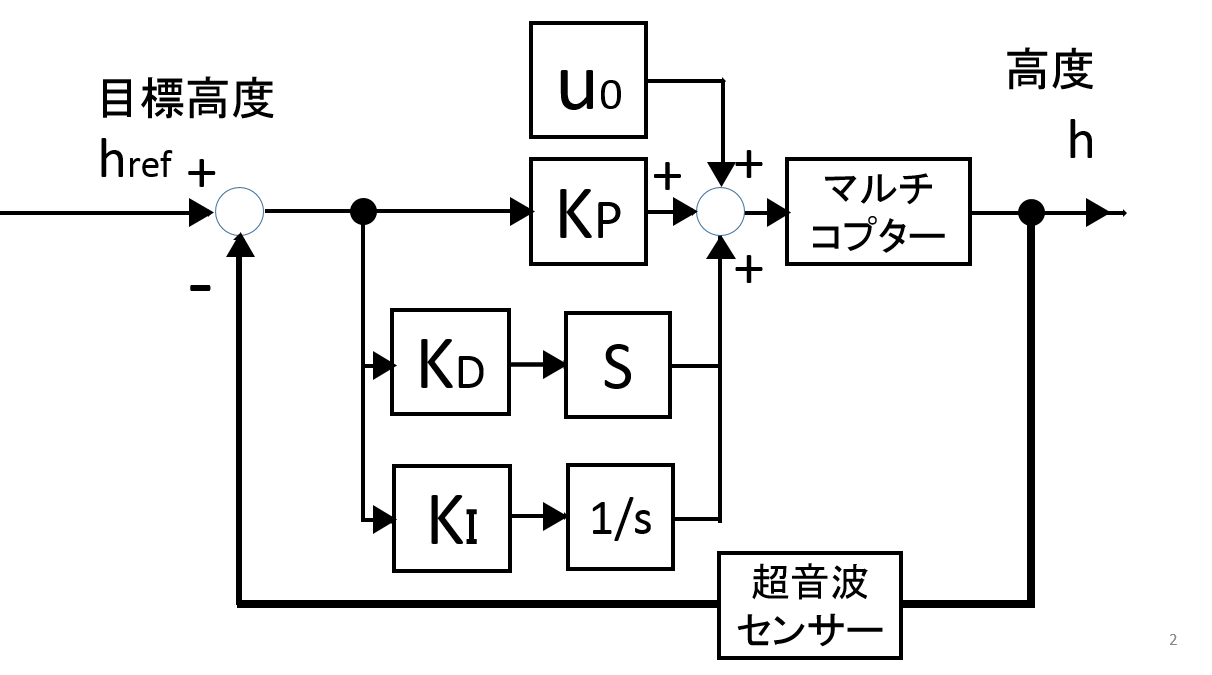
\includegraphics[width=150mm]{img/ブロック線図.png}
    \end{center}
  \caption{ブロック線図}
 \label{fig:ensyu3tex}
\end{figure}


目標高度 $h_{ref}$

実際の高度 h

誤差 e

とすると,

\begin{eqnarray}
e=h_{ref}-h
\end{eqnarray}

PID制御とは,制御入力uを次式で与える制御方式である.

\begin{eqnarray}
u=K_P\large{e}+K_D \large{e}+K_I\int\large{e}dt+u_0
\end{eqnarray}

\begin{eqnarray}
eの微分 \dot{e} とeの積分∫\large{e}dtについては,実際のプログラムでは制御周期をΔtとして
\end{eqnarray}


\begin{eqnarray}
\dot{e}\fallingdotseq \frac{ e_n-e_{(n-1)}}{Δt}\\
\end{eqnarray}

\begin{eqnarray}
∫edt \fallingdotseq \sum e
\end{eqnarray}


ここで
$K_P$ :比例ゲイン 

$K_D$ :微分ゲイン

$K_I$ :積分ゲイン



\begin{enumerate}
  \item 比例制御のみの結果を図5.2に示す.
比例制御だけでは発散して,高度制御ができないことがわかる.


  \item 比例制御と微分制御の実験を行った結果を図5.3に示す.
微分制御を加えたことで,安定するが目標値に一致しないことがわかる.


  \item 積分制御を使った結果を図5.4に示す.
積分制御を加えたことで,目標値に一致していることがわかる.

\begin{figure}[htbp]
  \begin{center}
   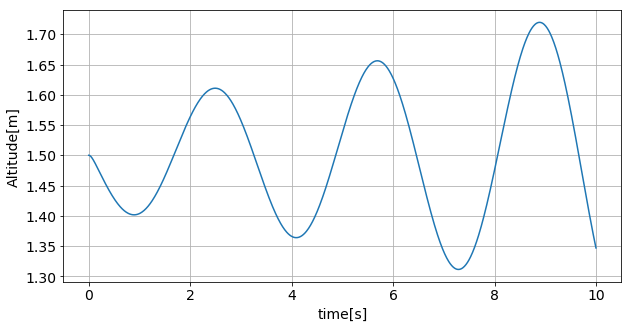
\includegraphics[width=150mm]{img/発散.jpg}
    \end{center}
  \caption{比例制御のみの高度結果}
 \label{fig:ensyu3tex}
\end{figure}

\begin{figure}[htbp]
  \begin{center}
   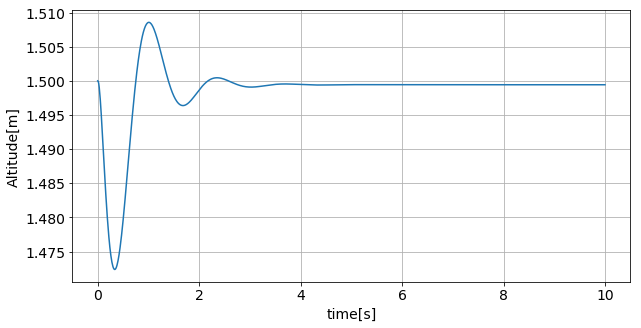
\includegraphics[width=150mm]{img/PD.jpg}
    \end{center}
  \caption{比例制御,微分制御の高度結果}
 \label{fig:ensyu3tex}
\end{figure}

\begin{figure}[htbp]
  \begin{center}
   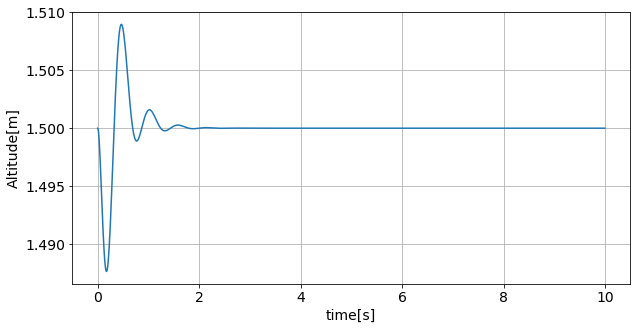
\includegraphics[width=150mm]{img/PIDbest.jpg}
    \end{center}
  \caption{比例制御,微分制御,積分制御の高度結果}
 \label{fig:ensyu3tex}
\end{figure}

\end{enumerate}


\chapter{考察}
図5.2より比例制御だけではマルチコプターが上下に発散して,高度制御ができないことがわかる.次に図5.3より比例制御に微分制御を加えたことで,安定するが目標値に一致しないことがわかる.最後に図5.4より比例制御と微分制御に積分制御を加えたことで,目標値に一致していることがわかる.これらの図より,初めに落ちてしまっている.これは1メモリ0.01mなので実際には約10mmしか落ちないので,あまり影響がないと考える.